%%
%% This is file `sample-sigconf.tex',
%% generated with the docstrip utility.
%%
%% The original source files were:
%%
%% samples.dtx  (with options: `sigconf')
%% 
%% IMPORTANT NOTICE:
%% 
%% For the copyright see the source file.
%% 
%% Any modified versions of this file must be renamed
%% with new filenames distinct from sample-sigconf.tex.
%% 
%% For distribution of the original source see the terms
%% for copying and modification in the file samples.dtx.
%% 
%% This generated file may be distributed as long as the
%% original source files, as listed above, are part of the
%% same distribution. (The sources need not necessarily be
%% in the same archive or directory.)
%%
%% The first command in your LaTeX source must be the \documentclass command.
\documentclass[sigconf]{acmart}

\usepackage{listings}
\usepackage{xcolor}
\usepackage{hyperref}
\usepackage{calc}
\usepackage{enumitem}

\lstdefinelanguage{JavaScript}{
  keywords={typeof, new, true, false, catch, function, return, null, catch, switch, var, if, in, while, do, else, case, break},
  keywordstyle=\color{blue}\bfseries,
  ndkeywords={class, export, boolean, throw, implements, import, this},
  ndkeywordstyle=\color{darkgray}\bfseries,
  identifierstyle=\color{black},
  sensitive=false,
  comment=[l]{//},
  morecomment=[s]{/*}{*/},
  commentstyle=\color{purple}\ttfamily,
  stringstyle=\color{red}\ttfamily,
  morestring=[b]',
  morestring=[b]"
}

\lstdefinelanguage{Golang}%
  {morekeywords=[1]{package,import,func,type,struct,return,defer,panic,%
     recover,select,var,const,iota,},%
   morekeywords=[2]{string,uint,uint8,uint16,uint32,uint64,int,int8,int16,%
     int32,int64,bool,float32,float64,complex64,complex128,byte,rune,uintptr,%
     error,interface},%
   morekeywords=[3]{map,slice,make,new,nil,len,cap,copy,close,true,false,%
     delete,append,real,imag,complex,chan,},%
   morekeywords=[4]{for,break,continue,range,go,goto,switch,case,fallthrough,if,%
     else,default,},%
   morekeywords=[5]{Println,Printf,Error,Print,},%
   sensitive=true,%
   morecomment=[l]{//},%
   morecomment=[s]{/*}{*/},%
   morestring=[b]',%
   morestring=[b]",%
   morestring=[s]{`}{`},%
}

\lstset{basicstyle=\ttfamily,breaklines=true}
\lstset{framextopmargin=50pt}


\newcommand{\todo}[1]{}
\renewcommand{\todo}[1]{{\color{red}{#1}}}
\newcommand{\bb}{\texttt{bigbro}~}
\newcommand{\bbheat}{\texttt{bbheat}~}
\newcommand{\bbstat}{\texttt{bbstat}~}

%% Rights management information.  This information is sent to you
%% when you complete the rights form.  These commands have SAMPLE
%% values in them; it is your responsibility as an author to replace
%% the commands and values with those provided to you when you
%% complete the rights form.
\setcopyright{acmcopyright}
\copyrightyear{2021}
\acmYear{2021}
\acmDOI{10.1145/1122445.1122456}

%% These commands are for a PROCEEDINGS abstract or paper.
\acmConference[SIGIR '21]{SIGIR '21: ACM SIGIR Conference on Research and Development in Information Retrieval}{June 03--05, 2021}{Woodstock, NY}
\acmBooktitle{SIGIR '21: ACM SIGIR Conference on Research and Development in Information Retrieval June 03--05, 2021, Woodstock, NY}
\acmPrice{15.00}
\acmISBN{978-1-4503-XXXX-X/18/06}


%%
%% Submission ID.
%% Use this when submitting an article to a sponsored event. You'll
%% receive a unique submission ID from the organizers
%% of the event, and this ID should be used as the parameter to this command.
%%\acmSubmissionID{123-A56-BU3}

%%
%% The majority of ACM publications use numbered citations and
%% references.  The command \citestyle{authoryear} switches to the
%% "author year" style.
%%
%% If you are preparing content for an event
%% sponsored by ACM SIGGRAPH, you must use the "author year" style of
%% citations and references.
%% Uncommenting
%% the next command will enable that style.
%%\citestyle{acmauthoryear}

%%
%% end of the preamble, start of the body of the document source.
\begin{document}

%%
%% The "title" command has an optional parameter,
%% allowing the author to define a "short title" to be used in page headers.
\title{\textit{Big Brother}: A Drop-In Website Interaction Logging Service}

%%
%% The "author" command and its associated commands are used to define
%% the authors and their affiliations.
%% Of note is the shared affiliation of the first two authors, and the
%% "authornote" and "authornotemark" commands
%% used to denote shared contribution to the research.
\author{Harrisen Scells}
\email{h.scells@uq.net.au}
\affiliation{%
  \institution{The University of Queensland}
  \city{Brisbane}
  \country{Australia}
}

\author{Jimmy}
\email{jimmy@ubaya.ac.id}
\affiliation{%
	\institution{University of Surabaya}
	\city{Surabaya}
	\country{Indonesia}
}

\author{Guido Zuccon}
\email{g.zuccons@uq.edu.au}
\affiliation{%
	\institution{The University of Queensland}
	\city{Brisbane}
	\country{Australia}
}

%%
%% The abstract is a short summary of the work to be presented in the
%% article.
\begin{abstract}
Fine-grained logging of interactions in user studies is important for studying user behaviour, among other reasons. However, in many research scenarios, the way interactions are logged is usually tied to a monolithic system. We present a generic, application-independent service for logging interactions in web-pages, specifically targetting user studies. Our service, Big Brother, can be dropped-in to existing user interfaces with almost no configuration required by researchers. Big Brother has already been used in several user studies to record interactions in a number of user study research scenarios, such as lab-based and crowdsourcing environments. We further demonstrate the ability for Big Brother to scale to very large user studies through benchmarking experiments. Big Brother also provides a number of additional tools for visualising and analysing interactions.

Big Brother significantly lowers the barrier to entry for logging user interactions by providing a minimal but powerful, no configuration necessary, service for researchers and practitioners of user studies that can scale to thousands of concurrent sessions. We have made the source code and releases for Big Brother available for download at \href{https://github.com/hscells/bigbro}{https://github.com/hscells/bigbro}.
\end{abstract}

%%
%% The code below is generated by the tool at http://dl.acm.org/ccs.cfm.
%% Please copy and paste the code instead of the example below.
%%
%\begin{CCSXML}
%<ccs2012>
% <concept>
%  <concept_id>10010520.10010553.10010562</concept_id>
%  <concept_desc>Computer systems organization~Embedded systems</concept_desc>
%  <concept_significance>500</concept_significance>
% </concept>
% <concept>
%  <concept_id>10010520.10010575.10010755</concept_id>
%  <concept_desc>Computer systems organization~Redundancy</concept_desc>
%  <concept_significance>300</concept_significance>
% </concept>
% <concept>
%  <concept_id>10010520.10010553.10010554</concept_id>
%  <concept_desc>Computer systems organization~Robotics</concept_desc>
%  <concept_significance>100</concept_significance>
% </concept>
% <concept>
%  <concept_id>10003033.10003083.10003095</concept_id>
%  <concept_desc>Networks~Network reliability</concept_desc>
%  <concept_significance>100</concept_significance>
% </concept>
%</ccs2012>
%\end{CCSXML}
%
%\ccsdesc[500]{Computer systems organization~Embedded systems}
%\ccsdesc[300]{Computer systems organization~Redundancy}
%\ccsdesc{Computer systems organization~Robotics}
%\ccsdesc[100]{Networks~Network reliability}

%%
%% Keywords. The author(s) should pick words that accurately describe
%% the work being presented. Separate the keywords with commas.
\keywords{user studies, interaction logging}



%%
%% This command processes the author and affiliation and title
%% information and builds the first part of the formatted document.
\maketitle

\section{Problem, Target Users \& Importance}

Recording interactions in a user study setting is extremely important for understanding user behaviour, among other reasons. However, writing the code to implement the recording of interactions can be tedious and a burden on those who wish to run user studies. Indeed, there is a considerable amount of software infrastructure to be considered when logging user interactions: How to efficiently process streams of interactions from multiple users/sessions? How to store the logs? How to deal with all the types of interactions a user might make? When we encountered these questions, it was clear that a \textit{standard}, \textit{simple}, and \textit{drop-in} service was required. The requirement for the service to passively log interactions once loaded into a web page also provides a generic way to capture events from users no matter the framework or setting that the user study is run.
We present this service to the wider IR community as an Open Source tool, dubbed \textit{Big Brother}. An overview of the Big Brother architecture is presented in Figure~\ref{fig:overview}.

\begin{figure}
\centering
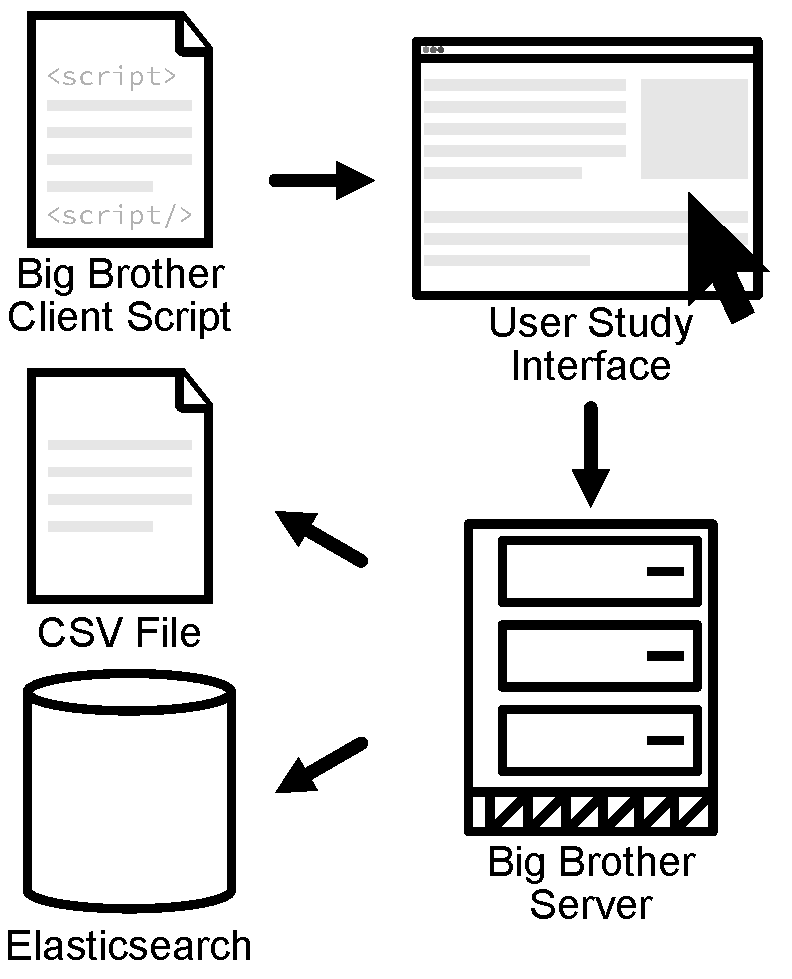
\includegraphics[width=0.76\linewidth]{overview}
\vspace{-4pt}
\caption{High-level overview of the system architecture.\vspace{-14pt}}
\label{fig:overview}
\end{figure}

%\section{Importance of System}

%Carefully designing an interface for user study experiments can be tedious and complicated. One consideration that is often overlooked, however, is tracking how users interact with a system. 
Fine-grained interaction logs enable researchers to more deeply understand how users behave in their systems. Tracking and analysing how users behave is important for a number of reasons:

\begin{description}
	\item[Evaluation] While self-reporting by users can provide a weak measure of effort required to complete tasks, tracking user interactions can provide a stronger source of evidence for how much effort, or how challenging a user found a task. For example, by logging user interactions, Cross et al.~\cite{cross2021search} found that user reported effort differed from the number of interactions between two systems.
	\item[User Modelling] Recording how users interact with systems enables a deeper understanding of user behaviour, and can lead to models that better reflect the needs of users. In Information Retrieval tasks, White~\cite{white2016interactions} notes that modelling user behaviour permits `better understanding the search process, estimating satisfaction, identify connections between queries and/or URLs, and learning which results are relevant.'
	\item[Multi-Modal Interactions] Often it is desirable to analyse behavioural patterns between how users interact with the keyboard and mouse and other physical interactions, such as a users emotions~\cite{arapakis2008affective}. For example Jimmy et al.~\cite{jimmy2020health} was able to better understand what users paid attention to by combining interaction data like clicks and mouse movements with eye-tracking.
	\item[Malicious Users] By tracking how frequently a user interacts with elements on a page it is possible to identify behavioural patterns that may correspond with malicious intent~\cite{gadiraju2015understanding}. Although, there have been no studies to date that are able to detect malicious behaviour automatically from user interactions alone.
\end{description}
\section{Operation of the System}

% What does your demonstration do and how does it work? What does it look like?

Big Brother has two main components: a high-throughput server and a JavaScript client. The client listens to events that occur in a web browser, and the server ingests them in real-time.
\vspace{-8pt}
\subsection{Client}

The Big Brother client has been written to provide maximum functionality with minimal setup and configuration. The smallest amount of code to have Big Brother listen to events is presented in Listing~\ref{lst:minimal}. By default, Big Brother is configured to listen to all events on all elements on a page. This client has been put to the test on multiple user studies with highly complex interfaces~\cite{cross2021search,jimmy2019health,jimmy2020health}. Practitioners of these studies and users of their systems noticed no slowdown of their study as a result of using Big Brother.

\begin{lstlisting}[language=JavaScript, label=lst:minimal, caption=Minimal example of code required to initialise \bb on the client-side. Note the \texttt{session\_id} which should already be initialised elsewhere.]
<script src="bigbro.js"></script>
<script type="text/javascript">
BigBro.init(session_id, "localhost:1984");
</script>
\end{lstlisting}

\noindent
Often, however, the practitioner of a user study may only be interested in a subset of events. Listing~\ref{lst:events} presents the JavaScript code required on the client-side to restrict Big Brother to listen to two events: \texttt{mousemove} and \texttt{onload}, which will record the coordinates of the users' mouse, and the time the session began respectively.

\begin{lstlisting}[language=JavaScript, label=lst:events, caption=Initialising \bb to listen on only certain global events. HTML code removed for brevity.]
BigBro.init(session_id, 
            "localhost:1984", 
            ["mousemove", "onload"]);
\end{lstlisting}

\noindent
Sometimes, the practitioner of a user study may wish to capture custom interactions or events from their user. For example, logging a custom event for when a user clicks a specific button on the page. Listing~\ref{lst:custom} presents the JavaScript code required on the client-side to wire the processing of a custom event to Big Brother's exposed custom logging functionality.

\begin{lstlisting}[language=JavaScript, label=lst:custom, caption=Wiring up \bb to listen to click events and to log a custom event.]
let bb = BigBro.init(session_id, 
                     "localhost:1984");
let w = window;
w.addEventListener("click", function (e) {
    bb.log(e, "custom_event");
})
\end{lstlisting}

\noindent
Finally, it is possible to record the screen using Big Brother. Listing~\ref{lst:capture} presents the minimum JavaScript code required to start a live capture of the browser window a user is looking at. Because of browser security, screen capture cannot be started automatically, and must be initiated by clicking an element (as seen in the argument provided to the function in Listing~\ref{lst:capture}). Captures are saved as a series of images. The time between each capture can be configured, and captures can be taken in response to events. The images can be stitched together into a video later, or can be used to highlight specific interactions from the logs. 

\begin{lstlisting}[language=JavaScript, label=lst:capture, caption=Wiring up \bb to listen to click events and to log a custom event.]
let bb = BigBro.init(session_id, 
                     "localhost:1984");
bb.startCaptureOnClick("capture");
\end{lstlisting}


The Big Brother client has been specifically designed to require very minimal configuration and setup. Likewise, the server is designed to be run independently of components such as the web server a user study is hosted on.


\subsection{Server}

The server is written in the Go programming language. This provides a number of advantages, primarily the ability for the server code to be compiled into a high-performance single-binary file for multiple platforms (macOS, Windows, Linux, etc.). The server can be configured using command-line options. It can also be integrated into existing web servers as library code, so long as those servers are written in Go.

\begin{table}
\centering
\begin{tabular}{p{0.2\linewidth}p{0.7\linewidth}}
\hline
Component & Description of Component \\
\hline
Target & The HTML element that has caused the event to trigger. \\
Name & The \texttt{name} attribute of the HTML element in Target. \\
ID & The \texttt{id} attribute of the HTML element in Target\\
Method & The name of the method that caused the event to trigger. \\
Location & The web-page location on the server (URL, with query string and anchors). \\
Comment & Any additional custom information that may be useful to interpreting the event. \\
X & The x-position within the web browser that the event occurred at. \\
Y & The y-position within the web browser that the event occurred at. \\
ScreenWidth & The width of the web browser the event occurred within. \\
ScreenHeight & The height of the web browser the event occurred within. \\
Time & The time the event happened.\\
Actor & An identifier that can be used to refer to the user that caused the event, e.g., session ID. \\
\hline
\end{tabular}
\caption{The components of an event.\vspace{-16pt}}
\label{tbl:event}
\end{table}

The server processes interactions from users as \textit{events}. The components that comprise an event are summarised in Table~\ref{tbl:event}.
An event captures information about the HTML elements that were interacted with (\textbf{Target}, \textbf{Name}, \textbf{ID}), how the event was triggered (\textbf{Method}), what the URL was on the page that the event occurred (\textbf{Location}), additional custom comments (\textbf{Comment}), positional information to "replay" interactions (\textbf{X}, \textbf{Y}, \textbf{ScreenWidth}, \textbf{ScreenHeight}), the time that the event occurred (\textbf{Time}), and the user that caused the event (\textbf{Actor}).

Events are streamed from the user's web browser to a centralised server over websockets. This enables the real-time ingestion of interactions. Currently, Big Brother can output logs to a local csv file as well as directly indexing them to Elasticsearch. A small, real example of logs captured during a user study is presented in Listing~\ref{lst:logs}. The researcher who ran this study decided to output their interaction logs directly to a csv file. The ordering of components in these events is how they are produced by \bb. Listing~\ref{lst:components} shows the ordering of components in the csv file output. These logs show the interactions of two user sessions from a human intelligence task (HIT) on a popular crowdsourcing platform. This slice of interaction logs begins when the \texttt{A1} user starts a HIT, and ends when they finish the HIT. At the same time, another user (\texttt{A2}) is in the middle of another HIT. The researcher running this user study records when their users click on a multiple select dropdown. The very final line in the log, when user \texttt{A1} finishes the HIT, also logs the recorded answers to the questionnaire using the Comment component: \texttt{T|T|T|T|T}.

In addition to allowing the researcher to see in real-time how users are interacting with their experiments (and potentially throw away sessions from users who completed the study too quickly), it provides a second way to record responses that users make to questionnaires.

\begin{figure*}
\vspace{-8pt}
\begin{lstlisting}[basicstyle=\footnotesize\ttfamily,caption=Example log file capturing two user sessions at the same time. Note that there were far more interactions captured during the study and that this is a small contrived slice of the data. Much of the information from the URL has been redacted.,label=lst:logs]
19-01-03 06:12:45,A1,hit_start,,,,https://example.com?assignmentId=XYZ123&hitId=HIT1,0,0,1319,646,
19-01-03 06:12:47,A1,click,SELECT,q1,,https://example.com?assignmentId=XYZ123&hitId=HIT1,1079,299,1319,646,
19-01-03 06:12:48,A1,click,SELECT,q1,,https://example.com?assignmentId=XYZ123&hitId=HIT1,0,0,1319,646,
19-01-03 06:12:49,A1,click,SELECT,q2,,https://example.com?assignmentId=XYZ123&hitId=HIT1,1067,328,1319,646,
19-01-03 06:12:46,A2,click,SELECT,q4,,https://example.com?assignmentId=ABC789&hitId=HIT2,806,233,1063,306,
19-01-03 06:12:46,A2,click,SELECT,q4,,https://example.com?assignmentId=ABC789&hitId=HIT2,0,0,1063,306,
19-01-03 06:12:50,A1,click,SELECT,q2,,https://example.com?assignmentId=XYZ123&hitId=HIT1,0,0,1319,646,
19-01-03 06:12:50,A1,click,SELECT,q3,,https://example.com?assignmentId=XYZ123&hitId=HIT1,1067,354,1319,646,
19-01-03 06:12:51,A1,click,SELECT,q3,,https://example.com?assignmentId=XYZ123&hitId=HIT1,0,0,1319,646,
19-01-03 06:12:49,A2,click,SELECT,q5,,https://example.com?assignmentId=ABC789&hitId=HIT2,779,260,1063,306,
19-01-03 06:12:52,A1,click,SELECT,q4,,https://example.com?assignmentId=XYZ123&hitId=HIT1,1069,390,1319,646,
19-01-03 06:12:50,A2,click,SELECT,q5,,https://example.com?assignmentId=ABC789&hitId=HIT2,0,0,1063,306,
19-01-03 06:12:53,A1,click,SELECT,q4,,https://example.com?assignmentId=XYZ123&hitId=HIT1,0,0,1319,646,
19-01-03 06:12:54,A1,click,SELECT,q5,,https://example.com?assignmentId=XYZ123&hitId=HIT1,1074,424,1319,646,
19-01-03 06:12:55,A1,click,SELECT,q5,,https://example.com?assignmentId=XYZ123&hitId=HIT1,0,0,1319,646,
19-01-03 06:12:56,A1,hit_end,INPUT,,submit,https://example.com?assignmentId=XYZ123&hitId=HIT1,659,617,1319,646,T|T|T|T|T
\end{lstlisting}
\vspace{-8pt}
\begin{lstlisting}[caption=Order of event components in Listing~\ref{lst:logs},label=lst:components]
	Time,Actor,Method,Target,Name,ID,Location,X,Y,ScreenWidth,ScreenHeight,Comment
\end{lstlisting}
\vspace{-8pt}
\end{figure*}

\vspace{-8pt}
\subsection{Throughput Benchmark}

We demonstrate the ability of Big Brother to scale and accommodate very large user studies by providing a throughput benchmark of logging user interactions directly to a csv file. To make the benchmark more realistic, we simulate the time it takes to process an event by encoding and decoding the event, and populate the event with random data. Each event has Target, Method, Location, X, Y, ScreenHeight, ScreenWidth, Time and Actor components. To benchmark the code, we use the standard benchmarking framework included in the Go language (as this is the language that the server is written in). In this framework, a loop containing the process described earlier is run $N$ times until it takes a second for the benchmark to complete. We report the total number of events processed, the average time it takes to process one event in microseconds, and the throughput in MB/s. We run the benchmark ten times and report both each run and the overall statistics. The benchmarks were run on a 2.7GHz Intel Core i7 8-core 2018 MacBook Pro with 16GB of LPDDR3 RAM and solid-state flash storage. Table~\ref{tbl:bench} presents the results of the benchmark. On average, Big Brother can process approximately 70,000 events per second, with each event processed in approximately 26$\mu$s, and write the interactions to a file at a speed of approximately 5MB/s. In practice, while we never came close to this amount of interactions per second, \bb did remain resilient and experienced no faults over the course of a number of studies.


\begin{table}
\centering
\begin{tabular}{p{0.28\linewidth}p{0.28\linewidth}p{0.29\linewidth}}
	\hline
	Processed Events    & $\mu$s/Event   & Throughput (MB/s) \\ \hline
	79,026     & 22.21          & 5.58              \\
	71,455     & 29.51          & 4.27              \\
	37,600     & 32.79          & 3.87              \\
	84,356     & 31.22          & 4.07              \\
	60,418     & 19.31          & 6.53              \\
	82,922     & 23.70          & 5.36              \\
	72,714     & 30.97          & 4.10              \\
	83,862     & 27.30          & 4.61              \\
	86,094     & 24.86          & 5.07              \\
	51,250     & 24.37          & 5.21              \\ \hline\hline
	70,969.70$\pm$16,326.29 & 26.60$\pm$0.27 & 4.87$\pm$0.34     \\ \hline
\end{tabular}
\caption{Benchmark results of logging events. The last row indicates average across the runs, with standard deviation. The processed events column indicates the number of events processed in one second.\vspace{-24pt}}
\label{tbl:bench}
\end{table}



\subsection{Other Tools within Big Brother}

The Big Brother family also includes other tools for visualising and manipulating data produced by the \bb tool. These include \bbheat and \bbstat, which are compatible with CSV formatted logs produced by \bb. If Elasticsearch is used as the storage medium for logs, it is possible to use the infrastructure that has been developed for it, including Kibana, a data visualization dashboard. Note that it is possible to use the Big Brother tools and the Elasticsearch tools by allowing \bb to write to a CSV file and ingesting that file into Elasticsearch using software such as Logstash. For details on how to use these tools, please refer to the GitHub repository.

\vspace{-8pt}
\subsection{\texttt{bbheat}}

\begin{figure}
	\vspace{-8pt}
	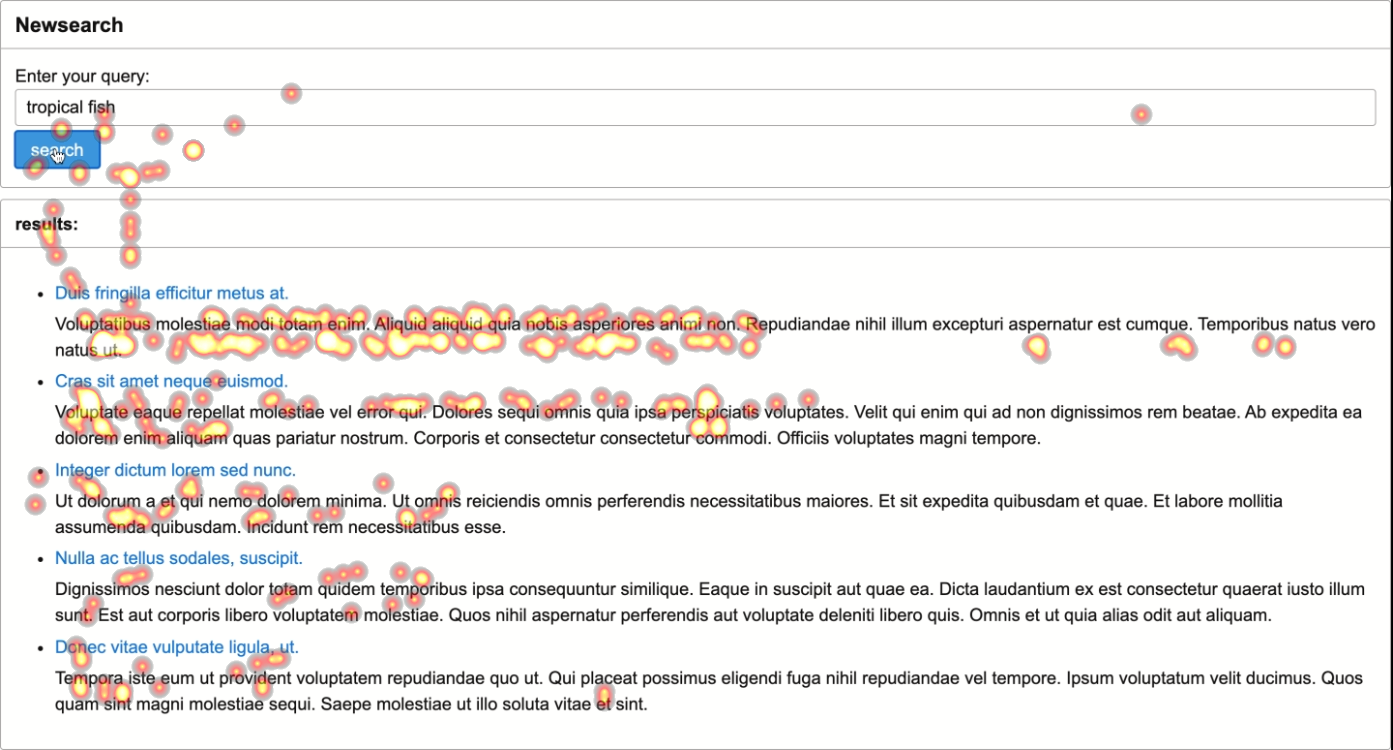
\includegraphics[width=\linewidth]{heatmap}
	\vspace{-8pt}
	\caption{Heat map of mouse interactions overlaid on top of an image of a search interface captured using the screen recording functionality of Big Brother.\vspace{-8pt}}
	\label{fig:heat}
\end{figure}

Often it is useful to be able to visualise the interactions of users over user interfaces. For this, the \bbheat tool can be used. This tool allows one to produce a static or animated heat map of mouse movements. The tool has several options for filtering interactions, for example by actor, time, and browser window size. An example of one of the heat maps produced by this tool is presented in Figure~\ref{fig:heat}. Using the screen recording functionality of Big Brother, it becomes trivial to visualise how different users interact with a system, or how changes in interface design can impact user behaviour.

\vspace{-8pt}
\subsection{\texttt{bbstat}}

Analysing log data can be tedious, especially processing the data for analysis. The \bbstat tool provides common functionality for processing interaction logs for later analysis. The functionality provided by the \bbstat tool include filtering: interaction logs can be split into multiple files based on actor, time, or comment, and aggregation: production of reports such as how long a user spent on different pages or how many times certain elements in a page were clicked.

\vspace{-8pt}
\subsection{Kibana}

Kibana is a product that is developed by the same company that built Elasticsearch. It provides tools for visualising and manipulating data. Kibana has been developed with time series logs in mind. A deeper description of Kibana is not provided here for space reasons, but it can be a powerful alternative to the tools provided by Big Brother.
\section{Comparison with Existing Systems}
\section{Impact of the System}


%%
%% The acknowledgments section is defined using the "acks" environment
%% (and NOT an unnumbered section). This ensures the proper
%% identification of the section in the article metadata, and the
%% consistent spelling of the heading.
\vspace{-8pt}
\small
\subsubsection*{Acknowledgements}
We would like to thank Anton van der Vegt and Sebastian Cross for their use of Big Brother in their user studies and Ahmed Mourad for proofreading a draft of this paper. Dr Guido Zuccon is the recipient of an Australian Research Council DECRA Research Fellowship (DE180101579) and Google Faculty Award. This research is supported by the Grain Research and Development Corporation (GRDC), project AgAsk (UOQ2003-009RTX).


%%
%% The next two lines define the bibliography style to be used, and
%% the bibliography file.
\bibliographystyle{ACM-Reference-Format}
\bibliography{sigir2021-bigbro-demo}


\end{document}
\endinput
%%
%% End of file `sample-sigconf.tex'.
